%%%%%%%%%%%%%%%%%%%%%%%%%%%% Define Article %%%%%%%%%%%%%%%%%%%%%%%%%%%%%%%%%%
\documentclass[nobib, openany, justified, a4paper, 14pt]{tufte-book}
%%%%%%%%%%%%%%%%%%%%%%%%%%%%%%%%%%%%%%%%%%%%%%%%%%%%%%%%%%%%%%%%%%%%%%%%%%%%%%%

%%%%%%%%%%%%%%%%%%%%%%%%%%%%% Citations %%%%%%%%%%%%%%%%%%%%%%%%%%%%%%%%%%%%%%%
%\usepackage[utf8]{inputenc}
\usepackage[style=authoryear-icomp]{biblatex}
%\usepackage[style=apa]{biblatex}
\addbibresource{/Users/ubd/Bibliotheca/bib.bib}
%%%%%%%%%%%%%%%%%%%%%%%%%%%%%%%%%%%%%%%%%%%%%%%%%%%%%%%%%%%%%%%%%%%%%%%%%%%%%%%

%%%%%%%%%%%%%%%%%%%%%%%%%%%%% Using Packages %%%%%%%%%%%%%%%%%%%%%%%%%%%%%%%%%%
\usepackage{newunicodechar}
\newunicodechar{🦜}{[parrot]}
\PassOptionsToPackage{prologue,dvipsnames}{xcolor}
\sloppy  % globally
\usepackage{geometry}
\usepackage{graphicx}
\usepackage{amssymb}
\usepackage{amsmath}
\usepackage{amsthm}
\usepackage{empheq}
\usepackage{mdframed}
\usepackage{booktabs}
\usepackage{lipsum}
\usepackage{graphicx}
\usepackage{color}
\usepackage{psfrag}
\usepackage{pgfplots}
\usepackage{bm}
\usepackage{epigraph}
\usepackage{titlesec}
\usepackage{tcolorbox}
\usepackage{csquotes}
\usepackage{pifont}
\usepackage{enumitem,amssymb}
% \usepackage{spoton} % adds \todo functionality I hope
%%%%%%%%%%%%%%%%%%%%%%%%%%%%%%%%%%%%%%%%%%%%%%%%%%%%%%%%%%%%%%%%%%%%%%%%%%%%%%%

% Other Settings

%%%%%%%%%%%%%%%%%%%%%%%%%% Page Setting %%%%%%%%%%%%%%%%%%%%%%%%%%%%%%%%%%%%%%%

%%%%%%%%%%%%%%%%%%%%%%%%%% Define some useful colors %%%%%%%%%%%%%%%%%%%%%%%%%%
\definecolor{maroon}{RGB}{128,0,0} %hlred
\definecolor{MAROON}{RGB}{128,0,0} %hlred
\definecolor{deepBlue}{RGB}{61,124,222} %url-links
\definecolor{deepGreen}{RGB}{26,111,0} %citations
\definecolor{ocre}{RGB}{243,102,25}
\definecolor{mygray}{RGB}{243,243,244}
\definecolor{shallowGreen}{RGB}{235,255,255}
\definecolor{shallowBlue}{RGB}{235,249,255}
\definecolor{mediumpersianBlue}{rgb}{0.0, 0.4, 0.65}
\definecolor{persianBlue}{rgb}{0.11, 0.22, 0.73}
\definecolor{persianGreen}{rgb}{0.0, 0.65, 0.58}
\definecolor{persianRed}{rgb}{0.8, 0.2, 0.2}
\definecolor{debianRed}{rgb}{0.84, 0.04, 0.33}
%%%%%%%%%%%%%%%%%%%%%%%%%%%%%%%%%%%%%%%%%%%%%%%%%%%%%%%%%%%%%%%%%%%%%%%%%%%%%%%

%%%%%%%%%%%%%%%%%%%%%%%%%% Indentation Settings %%%%%%%%%%%%%%%%%%%%%%%%%%%%%%%
\makeatletter
% Paragraph indentation and separation for normal text
\renewcommand{\@tufte@reset@par}{%
	\setlength{\RaggedRightParindent}{0pc}%1.0
	\setlength{\JustifyingParindent}{0pc}%1.0
	\setlength{\parindent}{1pc}%1pc
	\setlength{\parskip}{5pt}%0pt
}
\@tufte@reset@par

% Paragraph indentation and separation for marginal text
\renewcommand{\@tufte@margin@par}{%
	\setlength{\RaggedRightParindent}{0pc}%0.5pc
	\setlength{\JustifyingParindent}{0pc}%0.5pc
	\setlength{\parindent}{0.5pc}%
	\setlength{\parskip}{5pt}%0pt
}
\makeatother



%%%%%%%%%%%%%%%%%%%%%%%%%% Define an orangebox command %%%%%%%%%%%%%%%%%%%%%%%%
%o\usepackage[most]{tcolorbox}

\newtcolorbox{orangebox}{
	colframe=ocre,
	colback=mygray,
	boxrule=0.8pt,
	arc=0pt,
	left=2pt,
	right=2pt,
	width=\linewidth,
	boxsep=4pt
}


\newtcolorbox{redbox}{
	colframe=red,
	boxrule=0.8pt,
	arc=0pt,
	left=2pt,
	right=2pt,
	width=\linewidth,
	boxsep=4pt
}
%%%%%%%%%%%%%%%%%%%%%%%%%%%%%%%%%%%%%%%%%%%%%%%%%%%%%%%%%%%%%%%%%%%%%%%%%%%%%%%

%%%%%%%%%%%%%%%%%%%%%%%%%%%% English Environments %%%%%%%%%%%%%%%%%%%%%%%%%%%%%
\newtheoremstyle{mytheoremstyle}{3pt}{3pt}{\normalfont}{0cm}{\rmfamily\bfseries}{}{1em}{{\color{black}\thmname{#1}~\thmnumber{#2}}\thmnote{\,--\,#3}}
\newtheoremstyle{myproblemstyle}{3pt}{3pt}{\normalfont}{0cm}{\rmfamily\bfseries}{}{1em}{{\color{black}\thmname{#1}~\thmnumber{#2}}\thmnote{\,--\,#3}}
\theoremstyle{mytheoremstyle}
\newmdtheoremenv[linewidth=1pt,backgroundcolor=shallowGreen,linecolor=deepGreen,leftmargin=0pt,innerleftmargin=20pt,innerrightmargin=20pt,]{theorem}{Theorem}[section]
\theoremstyle{mytheoremstyle}
\newmdtheoremenv[linewidth=1pt,backgroundcolor=shallowBlue,linecolor=deepBlue,leftmargin=0pt,innerleftmargin=20pt,innerrightmargin=20pt,]{definition}{Definition}[section]
\theoremstyle{myproblemstyle}
\newmdtheoremenv[linecolor=black,leftmargin=0pt,innerleftmargin=10pt,innerrightmargin=10pt,]{problem}{Problem}[section]
%%%%%%%%%%%%%%%%%%%%%%%%%%%%%%%%%%%%%%%%%%%%%%%%%%%%%%%%%%%%%%%%%%%%%%%%%%%%%%%

%%%%%%%%%%%%%%%%%%%%%%%%%%%%%%% Plotting Settings %%%%%%%%%%%%%%%%%%%%%%%%%%%%%
\usepgfplotslibrary{colorbrewer}
\pgfplotsset{width=8cm,compat=1.9}
%%%%%%%%%%%%%%%%%%%%%%%%%%%%%%%%%%%%%%%%%%%%%%%%%%%%%%%%%%%%%%%%%%%%%%%%%%%%%%%

%%%%%%%%%%%%%%%%%%%%%%%%%%%%%%% MISC %%%%%%%%%%%%%%%%%%%%%%%%%%%%%%%%%%%%%%%%%%
\usepackage[acronym]{glossaries}
\usepackage{hyperref} % Setup: https://www.overleaf.com/learn/latex/Hyperlinks
\hypersetup{
	colorlinks=true,
	%citecolor=deepGreen,
	citecolor=maroon,
	linkcolor=persianBlue,
	filecolor=persianGreen,
	urlcolor=persianBlue,
	pdfpagemode=FullScreen,
}

%%%%%%%%%%%%%%%%%%%%%%%%%%%%%%%%%%%%%%%%%%%%%%%%%%%%%%%%%%%%%%%%%%%%%%%%%%%%%%%
\setcounter{tocdepth}{2}
\setcounter{secnumdepth}{2}

\newcommand{\hlred}[1]{\textcolor{Maroon}{#1}} % Print text in maroon
\newcommand{\hlgreen}[1]{\textcolor{persianGreen}{#1}} % Print text in green
\newcommand{\hlocre}[1]{\textcolor{ocre}{#1}} % Print text in green

\newenvironment{greenenv}{\color{Green}}{\ignorespacesafterend}  % Create green environment
\newenvironment{commentenv}{\color{ocre}}{\ignorespacesafterend}  % Create comment environment


\titleformat{\part}[display]
{\filleft\fontsize{40}{40}\selectfont\scshape}
{\fontsize{90}{90}\selectfont\thepart}
{20pt}
{\thispagestyle{epigraph}}

\setlength\epigraphwidth{.6\textwidth}

%\makeatletter
%\epigraphhead
%{\let\@evenfoot}
%{\let\@oddfoot\@empty\let\@evenfoot}
%{}{}
%\makeatother


%%%%%%%%%%%%%%%%%%%%%%%%%%%%%%%%%%%%%%%%%%%%%%%%%%%%%%%%%%%%%%%%%%%%%%%%%%%%%%%
%TODO LIST
\newlist{todolist}{itemize}{2}
\setlist[todolist]{label=$\square$}
\newcommand{\cmark}{\ding{51}}%
\newcommand{\xmark}{\ding{55}}%
\newcommand{\done}{\rlap{$\square$}{\raisebox{2pt}{\large\hspace{1pt}\cmark}}%
	\hspace{-2.5pt}}
\newcommand{\wontfix}{\rlap{$\square$}{\large\hspace{1pt}\xmark}}

%%%%%%%%%%%%%%%%%%%%%%%%%%%%%%%%%%%%%%%%%%%%%%%%%%%%%%%%%%%%%%%%%%%%%%%%%%%%%%%
\newcommand{\greensquare}{\marginnote{\fcolorbox{green}{green}{\rule{0pt}{3mm}\rule{3mm}{0pt}}\quad}}
\newcommand{\yellowsquare}{\marginnote{\fcolorbox{yellow}{yellow}{\rule{0pt}{3mm}\rule{3mm}{0pt}}\quad}}
\newcommand{\redsquare}{\marginnote{\fcolorbox{red}{red}{\rule{0pt}{3mm}\rule{3mm}{0pt}}\quad}}



\usepackage{epigraph}
\usepackage{titlesec}

\setcounter{tocdepth}{2}
\setcounter{secnumdepth}{2}

\newcommand{\hlred}[1]{\textcolor{Maroon}{#1}} % Print text in maroon

\titleformat{\part}[display]
  {\filleft\fontsize{40}{40}\selectfont\scshape}
  {\fontsize{90}{90}\selectfont\thepart}
  {20pt}
  {\thispagestyle{epigraph}}

\setlength\epigraphwidth{.6\textwidth}

\makeatletter
\xpatchcmd\epigraphhead
 {\let\@evenfoot}
 {\let\@oddfoot\@empty\let\@evenfoot}
 {}{}
\makeatother

%%%%%%%%%%%%%%%%%%%%%%%%%%%%%%% Title & Author %%%%%%%%%%%%%%%%%%%%%%%%%%%%%%%%
\title{\\ An \\ Anti-Liquefactionist \\Argument. \\\Large{Or why a consensus based AI assistance might not 
\\make demos any more democratic}}
\author{Utku B. Demir}
%%%%%%%%%%%%%%%%%%%%%%%%%%%%%%%%%%%%%%%%%%%%%%%%%%%%%%%%%%%%%%%%%%%%%%%%%%%%%%%

\begin{document}
    \maketitle
    \tableofcontents
    \newpage

\chapter*{Abstract}
This paper examines the impact of consensus-based cybernetic AI assistance on public deliberation and its potential effects on democratic quality. Drawing from post-structuralist analysis and engaging with concepts such as surveillance capitalism and the cyber republic, the study explores how AI systems designed to foster consensus in democratic processes may inadvertently undermine the pluralism and conflict essential for vibrant democratic engagement.%lorem ipsum
%
%\section{quotes}
%
%\begin{quote}
%  This paper examines the ways in which the institutionalization of surveillance capitalism has produced the deinstitutionalization of the democratic order through the erosion of informational, societal, behavioral and governance capabilities essential to democracy’s sustenance and reproduction\dots
%
%  -- \cite[5]{zuboff2022}
%
%\end{quote}
%
%\subsection{burroughs}
%
%\begin{quote}
%  A functioning police state needs no police.
%
%  -- \cite[23]{burroughs1992}
%  
%\end{quote}
%
%\subsection{zarkadakes}

%\begin{quote}
%  “A key concept worth exploring is a special state of equilibrium in complex systems called homeostasis. Again, the image of the flock of starlings is useful as a depiction of this special state. At any moment, the flock looks as if it is about to dissolve into its constituent parts, with single birds flying independently in all directions. And yet, the birds somehow regroup, and the flock continues its magnificent, fluid dance in the sky. This perilous dance at the edge of chaos is what homeostasis, a key characteristic of complex system behavior, looks like. Cybernetic systems exhibit such resilient behavior by using multiple feedback loops to reduce entropy and prevent themselves from decomposing under the second law of thermodynamics. Entropy is the degree of disorder in a system; the higher the entropy, the greater the disorder. ”
%  -- \cite[27]{zarkadakes2020}
%\end{quote}

%\begin{quote}
%The value of the massive-scale human-generated data obtained in stage one cannot be realized without computational systems of knowledge production known as machine learning and artificial intelligence. These systems, in turn, cannot perform without an everexpanding diet of massive-scale human generated data. The next step in the struggle for dominance over the politics of knowledge unfolds in stage two as data are transformed into information and knowledge with these proprietary computational ‘means of production’ along with the authority to determine what is produced, and who consumes it\dots
%\cite[28]{zuboff2022}
%  
%\end{quote}

\chapter{Introduction}

he increasing entanglement of artificial intelligence (AI) with the social landscape has introduced new challenges to the foundations of democracy. As AI systems evolve, they are playing an ever-greater role in shaping public discourse, influencing decision-making processes, and modulating social behavior. This growing influence raises critical questions: To what extent can AI be leveraged to enhance democracy and public deliberation? Can it contribute to more informed and inclusive public discourse, or does it risk reinforcing existing power structures, creating epistemic bubbles, and limiting the diversity of voices in the public sphere?

This paper first explores how the machinery of contemporary AI operates (focusing on the power structures it establishes within the framework of Gilles Deleuze's concept of the society of control) \parencite*{deleuze1992a}. Following an analysis of the social consequences of AI—specifically its role in shaping subjectivities and undermining democratic processes through the lens of thinkers such as Shoshana Zuboff \parencite*{zuboff2019}—the paper examines the potential and pitfalls of consensus-based cybernetic AI assistance in public deliberation, using George Zarkadakis' \parencite*{zarkadakes2020} concept of the Cyber Republic. The investigation focuses on whether these AI systems (which aim to facilitate democratic processes) inadvertently stifle the pluralism and factionalism necessary for democratic vitality.

By integrating insights from various scholars, the paper argues that while AI systems may streamline and enhance certain aspects of public deliberation, their tendency to promote consensus risks undermining the dynamic conflict that is essential for a healthy democracy. Rather than viewing entropy and discord as threats, this paper contends that these elements are critical for democratic renewal and should be preserved within AI-assisted deliberative processes. The \hlred{research question} is formulated with as follows:

\textit{ To what extent might the consensus-based cybernetic AI assistance for public deliberation in communities increase democratic quality?}

Furthermore, the research question will be examined via the following
hyptotheses: 

\hlred{Hypothesis 1:} Public deliberation is more likely to suffer from lack of diffusion in a consensus oriented cybernetic system.

\hlred{Hypothesis 2:} Consensus based cybernetic assistance more likely to
create epistemic bubbles through convergence.

\hlred{Hypothesis 3:} Communities that are assisted with a consensus based
cybernetic system are more likely to lose their factionalization ability.


\chapter{Control and Democracy}

The rapid advancements in artificial intelligence (AI) compel us to fundamentally rethink the core aspects of democracy: its definition, mechanisms, and inherent vulnerabilities. Rather than merely adapting democracy to mitigate the threats posed by AI, we must recognize that a transformation of democratic structures is both inevitable and essential for their survival and evolution. AI, far from being a neutral technology, has exacerbated many of the pre-existing challenges within our democratic systems, such as inequality, exclusion, and the degradation of public discourse. As a result, the resilience of democracy in this technological era demands more than just defensive measures; it requires a reimagining of democratic principles, reinvigorating the ideals of public deliberation, social communication, and civic participation that were championed during the Enlightenment and the revolutions that shaped modern republican values \parencite[see]{coeckelbergh2024}.

Current debates surrounding AI often center on how algorithms shape our subjectivities, public discourse, and democracy itself. As we look toward an AI-driven future, one crucial question arises: could the development of AI have followed a different path, one that better aligns with democratic ideals? However, before we address how to mitigate or resolve the issues that AI may exacerbate, we must first confront a more fundamental concern: what power structures do these algorithms inherently reinforce or establish? AI algorithms are not mere tools; they function as mechanisms that create and sustain networks of power. To truly grasp the implications of AI for democracy, we must critically analyze how these systems influence the production, dissemination, and control of knowledge, shaping the very foundation of public deliberation, civic engagement, and the production of subjectivity.
%%%%%%%%%%%%%%%

\section{Moles to Modulation, Discipline to Control}

%TODO: FOUCAULT
\epigraph{
  Power is everywhere; not because it embraces everything, but because it comes from everywhere. 

  -- \cite[93]{Foucault1978}
}
%Foucault's initial conceptualization of the disciplinary society and its \textit{governmentality} includes a non-monolithic type of power that operates in contrast to a sovereign society, not necessarily depending on violence but primarily through its knowledge of \textit{bodies}. This power can be direct, physical, calculating, and organized; but also technically thought out, subtle, and may make no use of weapons or terror, yet still maintains a physical order \parencite[25-26]{Foucault1995}.
%
%But disciplinary power, in the end, is generated within enclosures through the methodology of surveillance. Although internalized by the subject, it is still applied from one enclosure to another, from institution to institution, starting with the family, "to concentrate, to distribute, to compose a productive force" \parencite[3]{deleuze1992a}. It is no surprise that Foucault's analogy for disciplinary power was the \textit{panopticon} \parencite[see]{Foucault1995}, a mechanism that subjects individuals to the idea of constant surveillance, even when it is not actively enforced. Disciplinary power works efficiently to ensure that its subjects operate with maximum \textit{productivity}.
%
%\begin{quote}
%  Enclosures are molds, distinct castings, but controls are a modulation, like a self-deforming cast that will continuously change from one moment to the other, or like a sieve whose mesh will transmute from point to point.
%  
%  -- \cite[4]{deleuze1992a}
%\end{quote}
%
%Disciplinary societies exerted power through the control of bodies, relying on biopolitical methodologies to increase efficiency. The factory, the quintessential enclosure of the disciplinary society, focused on maximizing production while minimizing returns for the workers. The factory, the characteristic enclosure of the disciplinary society is simple
%point of intensity geared towards highest production with the least amount of
%yield for the workers; the mode of operation for the control society is the
%corporation. The corporation rather benefits from the motivational force that makes the
%individuals compete against each other subjecting them to a \textit{modulation}
%process
%\parencite[see 4]{deleuze1992a}. While the disciplinary society is discrete, moving individuals through distinct enclosures like family, school, barracks, and factory, the control society is continuous. Individuals are reduced to \textit{dividuals}, fragmented into data stored in \textit{banks}, where their bodies and identities are dissected, reassembled, and constantly visible across a network. Data particles combine in various ways to define the individual as a student, worker, or citizen. Traditional analogical spaces—family, school, army—are no longer distinct; they converge under a single owner. Man is no longer enclosed but indebted \parencite[see 5]{deleuze1992a}, perpetually reshaped to fit into imposed molds.
%
%\begin{quote}
%  The subject must not realize that the mistreatment is a deliberate attack of an anti-human enemy on his personal identity. He must be made to feel that he deserves any treatment he receives because there is something (never specified) horribly wrong with him. The naked need of the control addicts must be decently covered by an arbitrary and intricate bureaucracy so that the subject cannot contact his enemy direct.
%
%  -- Dr. Benway \parencite[17]{burroughs1992}
%  
%\end{quote}
%
%% Annexia, its Nazi mask and brutal state of terror, by then surpassed; the
%% Bismarck Archipelago, a pale European matriarchal democracy, on the style of
%% Great Britain, where deviances of several kinds are illegal and end up
%% assuming political relevance; and finally Freeland Republic, perhaps the most
%% dangerous of all, hypocrite, corrupt and obscure because it is active and it
%% tolerates all differences, but it then manipulates them for its own interest
%% of idealized supremacy through a repeated double game – Deleuze would define
%% it as “the axiomatics of capital immanence”. 27
%
%Deleuze adopts the concept of \textit{control} from William S.
%Burroughs \parencite*{burroughs1992} to describe this new operation of power.
%Burroughs' most well known Work \textit{Naked Lunch}\parencite*{burroughs1992} is a dissected dadaist
%exploration of the control via cut-up scenes roughly glued to each other. He
%believed that the cybernetical aproaches was the new operation of power which
%would carry out the control and manipulation in the western societies to shape
%them into a \textit{regularized entity} \parencite[see 18]{capitalism2018}.
%Naked Lunch's pratoganist William Lee (an alter ego of Burroughs) is
%accompanying us through different countries, Annexia, Interzone, Freeland
%\ldots. These countries are getting operated by different types of power whereas
%the Freeland is being where a perverse form of \textit{Control} is being
%engineered, and the character Dr. Benway is playing the embodiment of this new form of power. There
%are 4 different political parties in the book; Liquefactionists, Divisionists,
%Factualists and Conferents with Conferents being the control fanatics. A
%particularly intresting other group, the
%Liquefactionists are the ones supporting of humanity becoming one single body
%both figuratively and literally, one unified mind and body.

Foucault's initial conceptualization of the disciplinary society and its \textit{governmentality} includes a non-monolithic type of power that operates in contrast to a sovereign society, not necessarily depending on violence but primarily through its knowledge of \textit{bodies}. This power can be direct, physical, calculating, and organized; but also technically thought out, subtle, and may make no use of weapons or terror, yet still maintains a physical order \parencite[25-26]{Foucault1995}.

Disciplinary power, however, is generated within enclosures through the methodology of surveillance. Although internalized by the subject, it is still applied from one enclosure to another, from institution to institution, starting with the family, "to concentrate, to distribute, to compose a productive force" \parencite[3]{deleuze1992a}. Foucault's analogy for disciplinary power was the \textit{panopticon} \parencite[see]{Foucault1995}, a mechanism that subjects individuals to the idea of constant surveillance, even when it is not actively enforced. This system maximizes productivity by ensuring subjects operate efficiently and obediently within the bounds of the institution.

\begin{quote} Enclosures are molds, distinct castings, but controls are a modulation, like a self-deforming cast that will continuously change from one moment to the other, or like a sieve whose mesh will transmute from point to point.

-- \cite[4]{deleuze1992a} \end{quote}

While disciplinary societies relied on the control of bodies through fixed institutions like factories or schools, Deleuze describes a shift to societies of control. Here, power operates not through rigid enclosures but through continuous modulation. The factory, the characteristic enclosure of the disciplinary society, focused on maximizing production while minimizing returns for the workers. In contrast, the control society replaces the factory with the corporation, where individuals are no longer confined to static roles but instead subjected to a perpetual process of competition and self-regulation within fluid, dynamic networks. Control is no longer about disciplining bodies in specific spaces but about managing individuals through modulation—an ongoing process that shapes behavior and desires in real-time \parencite[see 4]{deleuze1992a}.

In disciplinary societies, individuals move from one enclosure to another (family, school, barracks, factory) where each institution molds them anew. However, control societies operate continuously; individuals are fragmented into \textit{dividuals}, reduced to data points within networks, where their identities are perpetually reassembled and monitored. The boundaries between traditional institutions blur, with spaces like family, school, and workplace converging under a corporate or state owner. Individuals are no longer enclosed but indebted, constantly reshaped to fit into fluid molds dictated by the demands of capital and digital networks \parencite[see 5]{deleuze1992a}.

\begin{quote} The subject must not realize that the mistreatment is a deliberate attack of an anti-human enemy on his personal identity. He must be made to feel that he deserves any treatment he receives because there is something (never specified) horribly wrong with him. The naked need of the control addicts must be decently covered by an arbitrary and intricate bureaucracy so that the subject cannot contact his enemy direct.

-- Dr. Benway \parencite[17]{burroughs1992} \end{quote}

Deleuze builds on William S. Burroughs’ concept of control to describe this new form of power. Burroughs’ novel \textit{Naked Lunch} \parencite*{burroughs1992} portrays control as a decentralized yet pervasive force, manifesting through a fragmented narrative style that mirrors the disjointed, fluid nature of modern power. Burroughs anticipated the cybernetic manipulation that would define Western societies, where control systems would gradually mold individuals into compliant entities, regularized through data and surveillance \parencite[see 18]{capitalism2018}.

In \textit{Naked Lunch}, Burroughs’ protagonist, William Lee, encounters various regimes of control across different territories, including Freeland, where a perverse form of control is engineered, embodied by the character Dr. Benway. Freeland, a place of apparent tolerance, uses difference and diversity as tools for manipulation and control, much like the systems Deleuze describes in societies of control. The political parties in the novel (Liquefactionists, Divisionists, Factualists, and Conferents) represent various forms of power, with the Conferents embodying control fanatics. Particularly intriguing are the Liquefactionists, who support the idea of humanity becoming one unified body, both figuratively and literally, a vision of control taken to its extreme, where individuality dissolves into collective unity. 


%\section{Residual Dividuals and Behavioral Surplus}
%
%% How is it all operationalised?
%
%\epigraph{[\ldots] controls are a modulation like a self-transmuting molding continually changing from one moment to the next, or like a sieve whose mesh varies from one point to another.
%
%  -- \cite[178-179]{Deleuze1995}
%}
%
%One might ask, but what is the operation of control. 
%
%Once vast data transfers became integral to the web, consumer data was no longer confined to discrete, time-bound moments. Instead, it began to flow continuously, creating a constant stream of real-time information based on web activity. The digital realm rapidly adapted to a market-driven structure, where user behaviors and characteristics became valuable assets to analyze and exploit for consumption patterns.
%A user's gender, location, and every single connection those surfing machines
%might establish has became the fundamental assets on the web. 
%
%%XXX: Intro Zuboff
%%TODO: Better place and edit this residual thema topic
%The digital became a surface whereas desiring-machines built connections and the
%surface became a criss-crossed entity 
%\sidenote{
%Here the internet is playing the role of both surface and a recording entity for
%a specific production process. Thus, it can be also argumented that it is a
%\textit{body without organs}, but its discussion is outside of the scope of this
%paper. See Deleuze and Guattari's description:
%
%\begin{quote}
%The body without organs, the unproductive, the unconsumable, serves as a surface for the recording of the entire process of production of desire, so that desiring-machines seem to emanate from it in the apparent objective movement that establishes a relationship between the machines and the body without organs
%-- \cite[11]{deleuze1983}
%\end{quote}
%
%} recording the remnants of human behavior. Hence, not all the human activity is
%directly related to the consumptional behavior, some completely irrelevant and
%minor data was labeled as \textit{residual data} in the beginning of the data
%reign. Let alone, being useful, the residual data was something to be get rid
%of, so the more useful data could shine. However, as the capabilities of the AI
%algorithms increased exponentially, their ability to scrutinise the residual
%data also increased leading to an untouched mines human behavior. This what
%Shoshana Zuboff \parencite*[see 74-82]{zuboff2019} labels as \textit{behavioral
%surplus} has become the main commodity
%of the surveillance capitalism, where the extraction of the behavioral
%commodity to sell the corporations is carried out by a pursuit to an ubiquotus
%data surveillance, the "product" is human behavior (see Figure \ref{fig:zuboff}) to predict and influence
%future behavior \parencite[71]{zuboff2019}. 
%
%
%\begin{marginfigure}
%  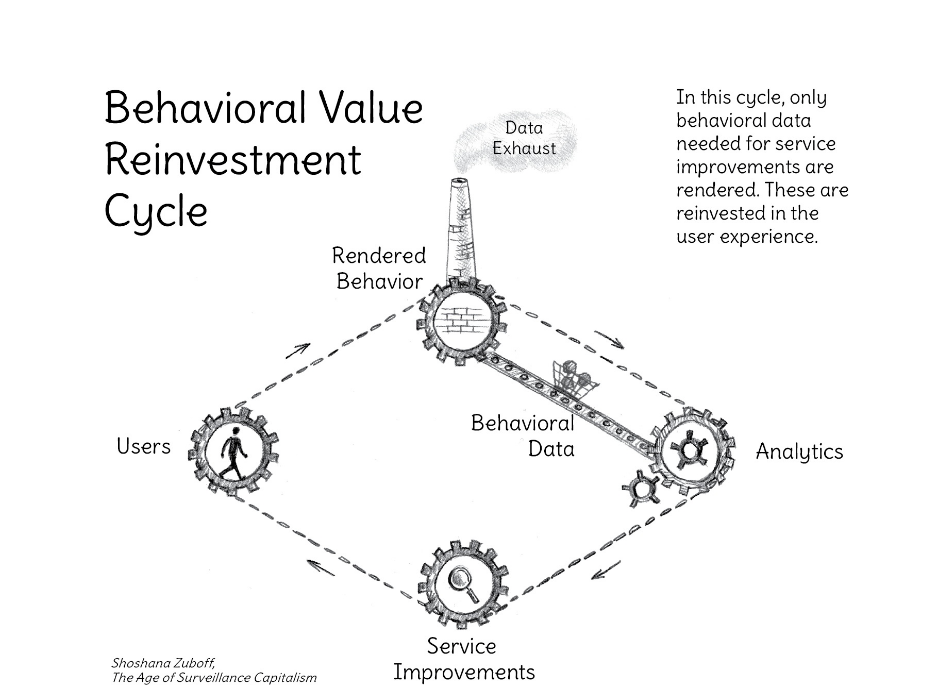
\includegraphics[scale=0.2]{zuboff.png}
%  \caption{The	Behavioral	Value	Reinvestment Cycle \parencite[72]{zuboff2019}}\\
%  \label{fig:zuboff}
%\end{marginfigure}
%
%Algorithmic processes employed by web analytics, online stores, social media platforms, and search engines analyze users' digital history and other residual data to build comprehensive profiles. Profiling individuals is just the first step in the methodology of the
%surveillance capitalism, both our intentionally stored data, as well as,
%residual data is lacking substance at the beginning, a comprehensive relevance
%assessment process is needed to build associations between behavioral patterns
%across the society to predict and possibly also manipulate human behavior. Once
%static and hierarchical categorization of human features are no more
%\parencite[see]{Gillespie2014}, the AI approaches in the surveillance capitalism
%Instead of placing users' data into fixed, predefined categories, algorithms
%operate in a fluid relationship with reality, continuously shaping and
%redefining categories based on the underlying logic of their design. As Cheney-Lippold \parencite*[170]{Cheney2011} points out, "algorithms allow a shift to a more flexible and functional definition of the category, one that de-essentializes gender from its corporeal and societal forms," while simultaneously re-essentializing it as "a statistically-related, largely market research-driven category". Gender as a category for example is no longer tied to biological or social norms but becomes a vector; a digital, math-based association shaped by market needs. This raises important questions about what norms mean for algorithmic systems, particularly when categories like gender are dynamically constructed to fit commercial interests. The categories that make up a user's profile are not static; they are constantly adjusted and redefined as new data about the user's behavior is collected. For instance, someone originally categorized as male could be recategorized as female if their recent online activity aligns more closely with \textit{algorithmically estimated} female behavior. This continuous feedback loop means that as more data flows in, the system refines its categorization. However, greater accuracy does not necessarily mean the digital classification will match the individual's real-world identity. In fact, categories like "maleness" are not based on fixed characteristics but are instead averages derived from the behavior patterns of a larger population, shaped by algorithmic analysis rather than real-world definitions. The categories are not carrying the purpose of mapping reality but to create the most effective and functional way to model (and predict) human behavior \parencite[135-145]{Cheney2011}.
%
%%TODO: Also introduce that we are bound to some kind of societal groups, again
%%fictional
%%TODO: Also remind that we are in a feedback loop
%%
%%TODO: Reality construction
%
%% ALTERNATIVE IST BELOW
%%This is "a	new	type	of	commerce	that	reimagines	us	through	the	lens	of	its	own distinctive	power,	mediated	by	its	means	of	behavioral	modification"\parencite[331]{zuboff2019}.  Through the data collection, profiling not only the commodities advertised to us are decided, the information we are getting, the social connections we are building are also steered by the algorithmic assessment of \textit{relevance}.
%%
%This new frontier of commerce reimagines individuals through the lens of behavioral modification, where data collection extends beyond surface-level actions to capture even the most intimate aspects of our inner lives, our emotions, preferences, and intentions. These pieces of personal information are transformed into countless data points, not for the purpose of improving well-being, but rather for calculation and profit \parencite[331]{zuboff2019}. However, algorithms determine not only the products advertised to us but also the information we are exposed to and the social connections we form. Everything is quantified and processed, fueling an industrial-like system where human behavior becomes the raw material for product development, marketing, and sales, and the flow of information operates in the same algorithmic governmentality. The social construction of the reality is inherent to the human experience, societies depend on the "commonsense knowledge" created collectively \parencite[42]{zuboff2022}, the social discourse in democracy is very much a product of the same process. Reality construction do not necessarily mean a society wide consensus, quite the contrary is democracy especially benefiting from the conjunctions and disjunctions 
%
%While the information individuals are getting governed by the algorithms by
%taking the digital tracks users leave in the digital realm, there is a constant
%adjustment of different \textit{relevance estimations}. How would it be
%estimated instead of what kind of shoes one likely to buy to what kind of
%political direction would suit them the best. The relevance here already becomes
%ambiguous, should one also gets associated to their specific political alignment
%and likely isolated from the other ones. One might argue for political safe
%spaces but the democracy does not benefit from isolation. Beyond the rationale
%of the association, the personalised reality construction process anchors us to
%multiple feedback loops. First, as previously noted, categories are dynamically
%updated as new data is processed. However, this category-level feedback loop is
%nonly one aspect of the anchoring mechanism—specifically, how algorithmic
%outcomes are tied to the user's prior actions. The second anchoring occurs
%between the subject's profile and the broader population with which the profile
%is categorized. The subject's digital environment, shaped by algorithms, is
%continually adjusted to align with the behaviors of these associated
%populations. In other words, the content the subject encounters is curated based
%on their past actions, but also tailored to fit the behavioral patterns of the
%group they are categorically linked to. Extending this process, a third feedback
%loop forms between the subject and their digital environment. As the content the
%subject consumes is filtered and personalized by the previous two anchoring
%systems, the subjectd’s thoughts and behaviors are increasingly shaped in
%alignment with the identities associated with their digital profile. This
%altered behavior, much like in a cybernetic loop reinforcing and normalizing the
%behavior in an ongoing loop \parencite[see 244-249]{Just2017}. At the end, as
%some kind of equlibrium is established between the current and the previous
%behavior of the individual, as well as, the group(s) they are associated with,
%an epistemic bubble establishes. Uer this analysis, there are the following
%emerging arguments about the contemporary algorithmic reality construction:


\section{Residual Dividuals and Behavioral Surplus}

\epigraph{[\ldots] controls are a modulation like a self-transmuting molding continually changing from one moment to the next, or like a sieve whose mesh varies from one point to another. -- \cite[178-179]{Deleuze1995}}

The question naturally arises: how does this operation of control actually function in the digital age?

With the rise of vast data transfers across the web, consumer data is no longer confined to discrete, time-bound events. Instead, it flows continuously, creating an unbroken stream of real-time information based on users' online activity. The digital realm rapidly conformed to a market-driven structure, where user behaviors and attributes became invaluable assets, not only to analyze but also to exploit for profit. Every element of a user’s online presence (gender, location, and every digital connection) became fundamental to this new economic model.

The digital became a surface whereas desiring-machines built connections and the
surface became a criss-crossed entity 
\sidenote{
Here the internet is playing the role of both surface and a recording entity for
a specific production process. Thus, it can be also argumented that it is a
\textit{body without organs}, but its discussion is outside of the scope of this
paper. See Deleuze and Guattari's description:

\begin{quote}
The body without organs, the unproductive, the unconsumable, serves as a surface for the recording of the entire process of production of desire, so that desiring-machines seem to emanate from it in the apparent objective movement that establishes a relationship between the machines and the body without organs
-- \cite[11]{deleuze1983}
\end{quote}

} recording the remnants of human behavior. Hence, not all the human activity is
directly related to the consumptional behavior, some completely irrelevant and
minor data was labeled as \textit{residual data} in the beginning of the data
reign. Initially, much of this "irrelevant" data was dismissed as \textit{residual data}, considered superfluous and discarded in favor of more useful information. However, as AI capabilities expanded exponentially, what was once residual became a treasure trove—a mine of untapped human behavior. This is what Shoshana Zuboff \parencite*[74-82]{zuboff2019} labels as behavioral surplus, a key commodity of surveillance capitalism. The pursuit of ubiquitous data surveillance transformed human behavior into a product—an asset to be extracted, analyzed, and sold to corporations with the sole purpose of predicting and influencing future actions \parencite[71]{zuboff2019}.

\begin{marginfigure} 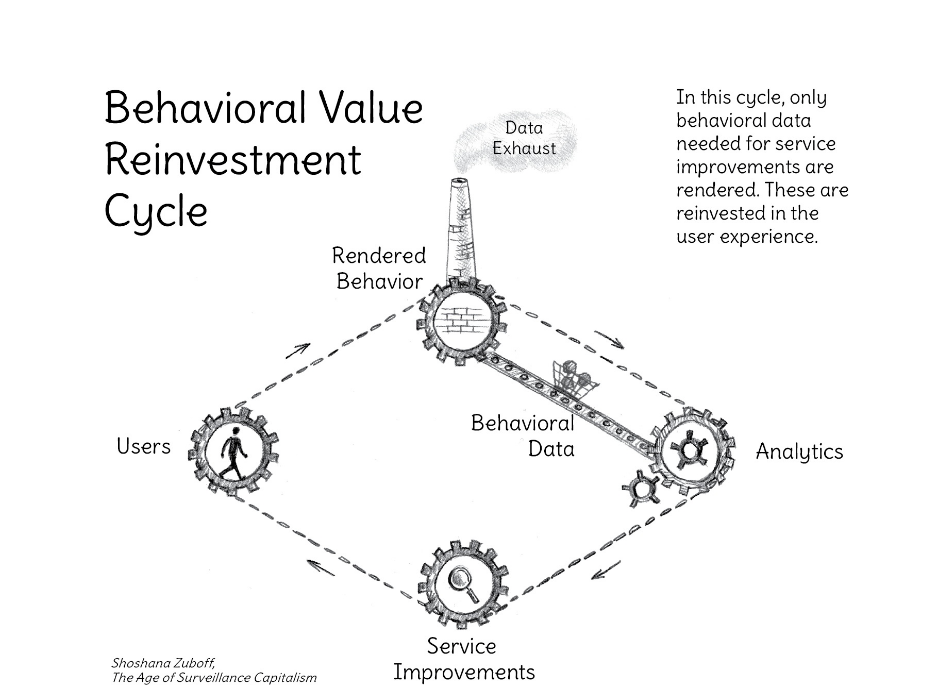
\includegraphics[scale=0.2]{zuboff.png} \caption{The Behavioral Value Reinvestment Cycle \parencite[72]{zuboff2019}}\ \label{fig
} \end{marginfigure}

Algorithmic processes, employed by platforms such as web analytics, online stores, social media, and search engines, systematically collect and scrutinize users' digital footprints, including both intentional and residual data. These algorithms don't merely store fixed user profiles; instead, they continuously refine and redefine categories based on evolving behavioral patterns. As Cheney-Lippold \parencite*[170]{Cheney2011} argues, algorithms enable a flexible and functional approach to categorization, de-essentializing concepts like gender from biological or social norms and re-essentializing them as vectors; digital, market-driven associations. These categories, shaped by the logic of capital, are not designed to reflect reality but to model human behavior for the most effective predictive and commercial outcomes.

In this ever-shifting algorithmic landscape, user profiles are not static. Categories are updated and recalibrated as new data streams in, resulting in a continuous feedback loop. This loop ensures that as user behavior evolves, the algorithm refines its categorization—yet, greater accuracy does not necessarily translate to a more truthful or authentic representation of the individual. Instead, profiles are abstracted into averages, shaped by the behavioral patterns of the populations to which the user is algorithmically assigned. The purpose is not to map reality, but to model, predict, and ultimately manipulate human behavior \parencite[135-145]{Cheney2011}.

This new frontier of commerce reimagines individuals through the lens of behavioral modification. Data collection extends beyond surface-level actions, capturing intimate aspects of human experience—emotions, preferences, and intentions. These elements of personal life are not collected for self-improvement, but for calculation and profit \parencite[331]{zuboff2019}. The products advertised to us, the information we are exposed to, and the social connections we make are all filtered through an algorithmic assessment of relevance. Reality, in this sense, is algorithmically constructed, not through consensus but through the selective reinforcement of behaviors that align with market interests. As Zuboff points out, this process governs not only what we consume but how we engage with the world.

While the information individuals receive is governed by algorithms that track the digital footprints users leave in the digital realm, there is a constant adjustment of different \textit{relevance estimations}. Rather than estimating what kind of shoes someone is likely to buy, algorithms estimate what political direction might suit them best. Here, relevance becomes ambiguous, as individuals are associated with specific political alignments and likely isolated from others. One might argue for political safe spaces, but democracy does not benefit from isolation. Beyond the rationale of association, the personalized reality construction process anchors individuals to multiple feedback loops.

First, as previously noted, categories are dynamically updated as new data is processed. However, this category-level feedback loop is only one aspect of the anchoring mechanism—specifically, how algorithmic outcomes are tied to the user's prior actions. The second anchoring occurs between the subject's profile and the broader population with which their profile is categorized. The subject's digital environment, shaped by algorithms, is continually adjusted to align with the behaviors of these associated populations. In other words, the content the subject encounters is curated based on their past actions and tailored to fit the behavioral patterns of the group to which they are categorically linked.

Extending this process, a third feedback loop forms between the subject and their digital environment. As the content the subject consumes is filtered and personalized by the previous two anchoring systems, the subject’s thoughts and behaviors are increasingly shaped in alignment with the identities associated with their digital profile. This altered behavior, much like in a cybernetic loop, reinforces and normalizes the behavior in an ongoing cycle \parencite[244-249]{Just2017}. In the end, as some form of equilibrium is established between the individual's current and past behavior, as well as the group(s) with which they are associated, an epistemic bubble is formed. Under this analysis, several key arguments emerge about the contemporary algorithmic construction of reality.

\section{A Cybernetic Alliance?}

The machinery of surveillance capitalism is deliberately designed and operated by private corporations. Zuboff's concept of \textit{instrumentarianism} names the deployers of this particular form of control as the puppet masters, whose aim is to modify, predict, monetize, and control human behavior \parencite*[331]{zuboff2019}. However, it doesn't necessarily address whether the machinery itself could be repurposed for different, more beneficial ends. A pressing question emerges: could we use algorithmic profiling, relevance association, and reality construction for the benefit of democracy and public discourse? Is there something inherently detrimental about AI algorithms operating on human data to \textit{personalize} societal exchange, or can these systems enrich democratic interaction without corrupting it, or we are doomed to be corrupted once we get to use the the power of the ring?        

George Zarkadakis \sidenote{While the Latinization of $\eta$ (eta) was traditionally rendered as an \textit{e} (e.g., Socrates), modern translations favor \textit{i} (e.g., Sokratis). Following this convention, the article refers to the author as Zarkadakis, not Zarkadakes.} \parencite*{zarkadakes2020} explores the possibility of building a cyber republic through AI-assisted small communities. Similar to the Helene Landemore's
\parencite*{landemore2020} \textit{mini  public} concept, Zarkadakis introduces \textit{citizen asssmblies} as participatory bodies that are designed to democratize decision-making by including citizens, particularly non-experts, in deliberation processes. These citizen assemblies combine direct democratic processes with representative governance, ensuring that citizens participate in decision-making both at regional and national levels. Citizen assemblies are supported by expert knowledge to combat misinformation and AI algorithms to manage the vast networks of information and communication (see Figure \ref{fig
}).

\begin{quote}
  “A key concept worth exploring is a special state of equilibrium in complex systems called homeostasis. Again, the image of the flock of starlings is useful as a depiction of this special state. At any moment, the flock looks as if it is about to dissolve into its constituent parts, with single birds flying independently in all directions. And yet, the birds somehow regroup, and the flock continues its magnificent, fluid dance in the sky. This perilous dance at the edge of chaos is what homeostasis, a key characteristic of complex system behavior, looks like. Cybernetic systems exhibit such resilient behavior by using multiple feedback loops to reduce entropy and prevent themselves from decomposing under the second law of thermodynamics. Entropy is the degree of disorder in a system; the higher the entropy, the greater the disorder. ”
  -- \cite[27]{zarkadakes2020}
\end{quote}

Zarkadakis heavily leans on the principles of cybernetics, a field first developed by Norbert Wiener \parencite*{Wiener1948}. Cybernetic systems display emergent behaviors due to the continuous communication between their parts, which occur through feedback loops. Output signals are often mixed with inputs from the environment or other parts of the system, and these are fed back into the system, creating recursive interactions. These feedback loops are critical, as they can alter the internal structure of the system itself. Take the human brain, for example, composed of billions of interconnected neurons. When the brain makes a decision (whether conscious or not), it processes signals from the senses and internal signals, continuously modifying the connections between neurons. Just as the brain is constantly reconfiguring itself in response to its environment, all cybernetic systems adapt through the continuous processing of multiple signals traveling within feedback loops \parencite[24]{zarkadakes2020}.

Zarkadakis proposes that democracy can be understood as a cybernetic system, where decentralized feedback loops between citizens and institutions drive societal change. He contrasts this vision with authoritarian regimes, which centralize decisions and use data to control populations. For cybernetic democracy to succeed, power must be distributed across a network of equal nodes, fostering resilience, participation, and individual freedom. Early iterations of the Internet aimed to achieve this, but the emergence of echo chambers in Web 2.0 highlights the danger of losing open democratic dialogue. Zarkadakis calls for a reimagining of democratic structures, utilizing AI to safeguard against exclusion, surveillance, and marginalization, ensuring that democracy evolves into a more inclusive and participatory system \parencite[25-27]{zarkadakes2020}.

\begin{marginfigure} 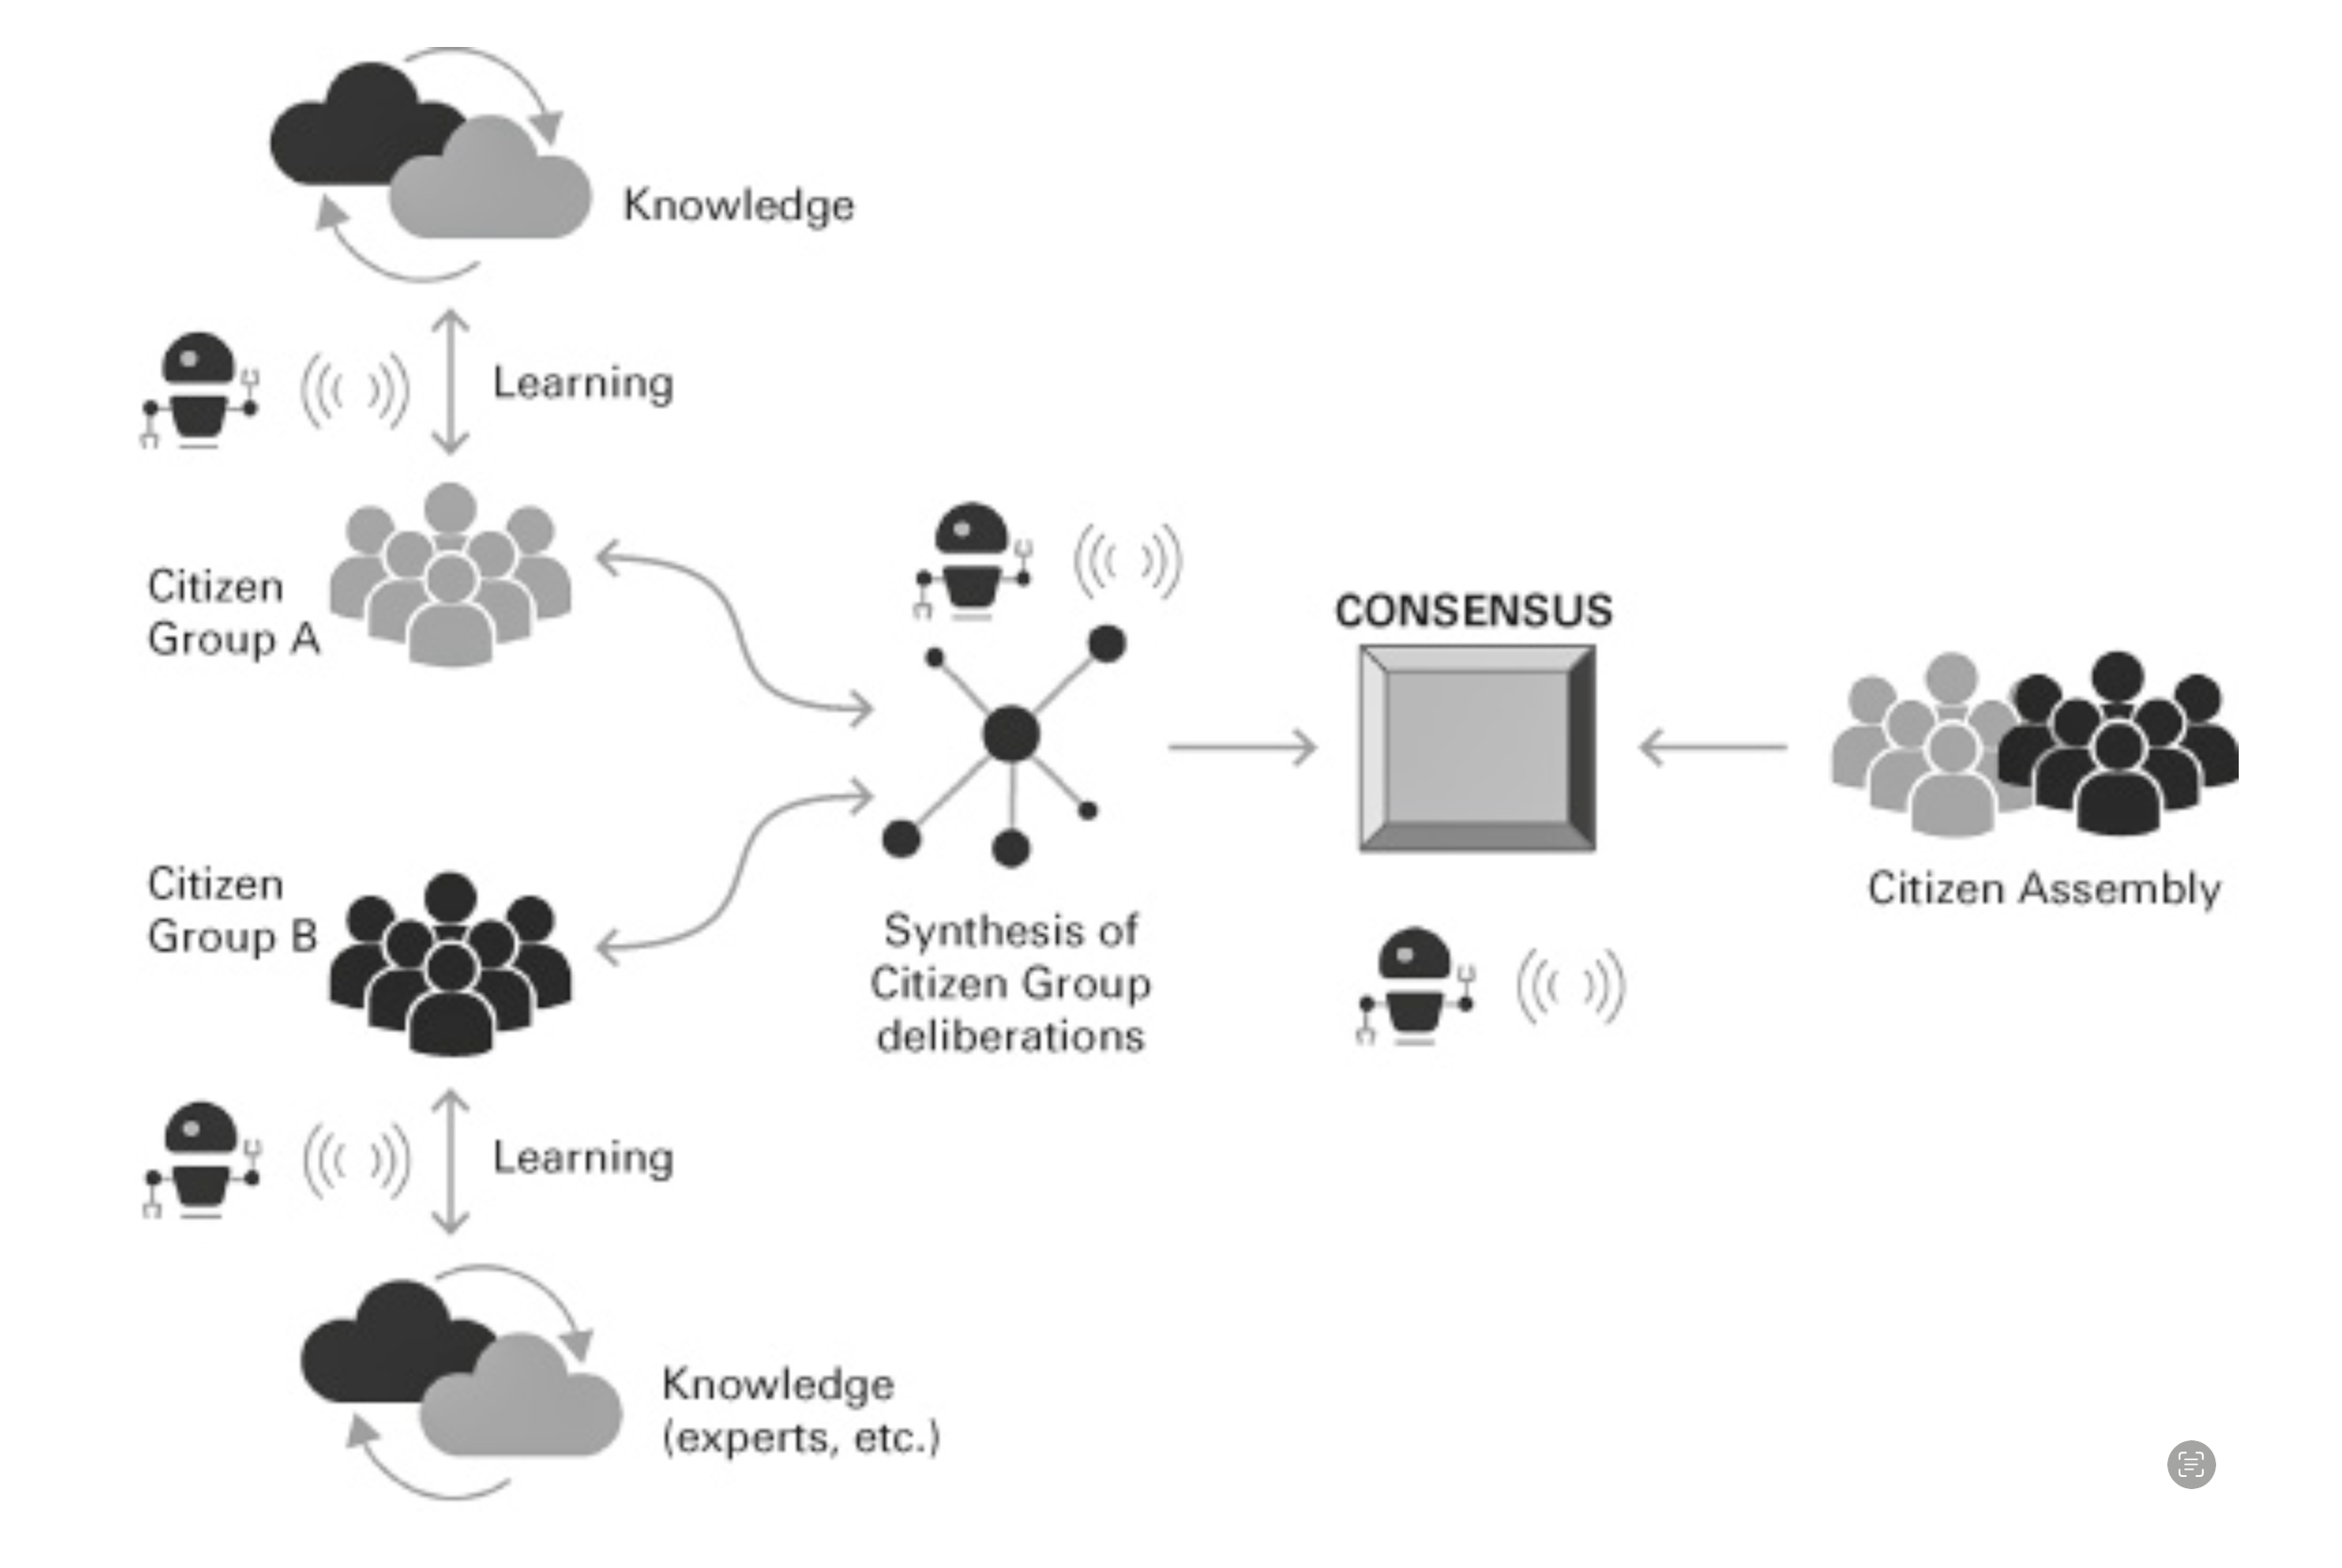
\includegraphics[scale=0.2]{zarkadakis.png} \caption{Using cybernetic conversational agents to facilitate a deliberative process while preserving humans in the loop. \parencite[43]{zarkadakes2020}}\ \label{fig:zarkadakis} \end{marginfigure}

Zarkadakis envisions a community that leverages the cybernetic feature of feedback loops to enhance human-machine communication. He elaborates on this collaboration by drawing on Gordon Pask's conversation theory, which posits that knowledge is co-constructed through dialogue between interacting agents, whether human or machine. This interaction is guided by feedback loops, which continuously reshape the internal structures of both participants. The knowledge generated from these interactions is captured in entailment meshes, which represent the evolving meaning and structure of the conversation. This cybernetic approach emphasizes adaptive, dynamic learning through interaction, demonstrating the critical role of recursive feedback in AI systems. Entailment meshes capture the evolving understanding between two participants. For the initiator (A), the mesh includes key topics and how they interrelate, referred to as "descriptive dynamics." For instance, if A discusses immigration, the mesh might include topics like "economic impact" or "multiculturalism." A also defines "prescriptive dynamics" by suggesting how these topics could form new concepts, like an "immigration policy." The second participant (B) interprets A’s mesh, reconstructs it from their own perspective, and provides feedback. Through ongoing adjustments, A and B refine their understanding, ultimately reaching a shared perspective for collaboration or decision-making \parencite[25-27]{zarkadakes2020}. 

\section{The Nomad and the Suffocating Unity}

\begin{quote} Cybernetic systems exhibit such resilient behavior by using multiple feedback loops to reduce entropy and prevent themselves from decomposing under the second law of thermodynamics. Entropy is the degree of disorder in a system; the higher the entropy, the greater the disorder. -- \cite[27]{zarkadakes2020} \end{quote}

Zarkadakis' solution begins with an ambitious assumption about the relationship between entropy and democracy. His entire algorithmic system rests on the perceived harm of disorder to democratic functioning. However, drawing on the radical democratic theory of Ernesto Laclau and Chantal Mouffe \parencite*{laclau1985}, one could argue that democracy actually thrives on a certain level of entropy and discord. Viewing democracy as a cybernetic system, equilibrium represents stagnation; just as in cybernetics, where a system reaches equilibrium by ceasing to adapt and evolve, democracy becomes inert without internal contradictions and debates. Deleuze and Guattari also contend that democracy cannot survive if the market remains its sole driving force. The subordination of public discourse to capital undermines the factionalism essential for democratic vitality, rendering deliberation hollow \parencite[see 176-178]{patton2020}. While Zarkadakis’ cybernetic model of consensus seeks harmony, it risks trapping individuals within the epistemic structures that current AI systems already reinforce \sidenote{\hlred{Hypothesis 1:} Public deliberation is more likely to suffer from a lack of diffusion in a consensus-driven cybernetic system.}.

\begin{quote} You see, control can never be a means to any practical end... It can never be a means to anything but more control... Like junk... -- \cite[81]{burroughs1992} \end{quote}

Zarkadakis' system includes measures such as expert mediation and topic diversity to address the lack of diffusion. However, its consensus-oriented nature still threatens the factionalism that sustains democracy. While the platform may provide a structured environment for exchanges mediated by experts, true democratic vitality depends on contradiction and dissent. Social movements offer striking examples: the Yellow Vest movement in France \parencite{hayat2022} and the Gezi Resistance in Turkey \parencite{tufekci2020} both collapsed before achieving their aims, partly because they rejected factionalism in favor of unity. Though these movements began with momentum, their insistence on unity ultimately stifled their progress. This lack of internal division led to their decline, illustrating how consensus, rather than strengthening movements, can suffocate the dynamism they require to thrive \sidenote{\hlred{Hypothesis 3:} Communities assisted by consensus-based cybernetic systems are more likely to lose their capacity for factionalization.}. Moreover, once equilibrium is achieved, the cybernetic system must defend this state by discouraging diffusion from established categories, potentially expanding or tightening control over discourse.

While societal implications are central, Zarkadakis' model also overlooks the individual dimension. The cybernetic framework offers little beyond the current systems of personalization and relevance filtering that already dominate reality construction. Despite its sophistication, this model still anchors individuals to pre-defined assessments of relevance. Personalization functions more as a reinforcement than a challenge. Except for expert interventions, the cybernetic equilibrium is likely to confine individuals within epistemic bubbles—consensus-driven, yet restrictive—limiting the potential for intellectual and ideological development \sidenote{\hlred{Hypothesis 2:} Consensus-based cybernetic assistance is more likely to create epistemic bubbles through convergence.}. This framework tends to encapsulate conflicts within broad categories, sacrificing the depth of discourse for the sake of stability and equilibrium.

Can a productive alliance between humans and algorithms exist within this framework? I argue that fostering individual diffusion, rather than unity, is essential for the emergence of democratic subjectivity. Deleuze and Guattari’s concept of the \textit{nomad} \parencite*{deleuze1983} offers a model. The nomad, as a desiring-machine, continuously forms new connections, often seemingly irrelevant or random across the social landscape. This nomadic movement provides an opportunity to escape the narratives imposed by dominant power structures \parencite[see 148]{deleuze1983}. How might an algorithm assist the nomad? By doing the opposite of what Zarkadakis' system proposes: instead of categorizing individuals into consensus-based groups, the algorithm should challenge subjectivity by exposing users to controversial and divergent information. Rather than striving for equilibrium, such a system would promote division and dynamic communication, allowing individuals to engage with multiple discourses, rather than being confined within epistemic bubbles. 

\chapter{Conclusion}

This paper has argued, while consensus-based cybernetic AI systems may streamline decision-making processes and foster more efficient public discourse, they come with significant risks. By promoting convergence and consensus, these systems may inadvertently stifle the pluralism, factionalism, and dissent that are essential for the health of democratic societies. Drawing from the insights of Deleuze’s concept of control, Zuboff’s critique of surveillance capitalism, and the radical democratic theories, this analysis demonstrates that democracy depends not on the elimination of conflict, but on its continual negotiation and expression.

Consensus-based AI systems risk reinforcing existing power structures and creating epistemic bubbles, thereby isolating individuals from the diversity of perspectives necessary for democratic renewal. As Zarkadakis’ cybernetic model highlights, AI assistance can facilitate public deliberation, but its focus on stability and homeostasis may lead to an erosion of the very dynamism that keeps democracy alive. True democratic participation requires systems that not only support deliberation but actively encourage conflict, contradiction, and the challenging of established categories.

In light of these findings, this paper advocates for a rethinking of AI's role in public deliberation. Rather than aiming for consensus, AI systems should be designed to foster division, diversity, and exposure to divergent viewpoints. A more nomadic approach—drawing on Deleuze and Guattari’s concept of the desiring-machine—offers a productive model for ensuring that AI systems support, rather than undermine, the democratic process. By prioritizing individual diffusion over collective unity, and by promoting dynamic interaction over static consensus, AI systems can help sustain the open, pluralistic dialogue that is the lifeblood of democracy.


\printbibliography
\end{document}
